\section{Model}

This section describes our model. We will start by describing a simplistic 
version of our model, and continue to introduce new properties until we reach 
the full model.

\subsection{Symbols}

This is a dummy section to introduce the symbols used later...

\begin{description}
 \item [$S$] the substrate tree with $S = (\SubstrateNodes, \SubstrateEdges)$
 \item [$\SubstrateNodes$]  a set of nodes: $\{\SubstrateNode_1, \dots , 
\SubstrateNode_{|\SubstrateNodes|}\}$
 \item [$\SubstrateNodes$] a set of edges : $\{\SubstrateNode_1, \dots , 
 \SubstrateEdge_{|\SubstrateEdge|}\}$ with $\SubstrateEdge_1 = 
(\SubstrateNode_i, \SubstrateNode_j)$
 \item [$c_i$] A chunk of type $i$
 \item [$v_i$] The i-th $\VM$ of the request
 \item [$\VirtualNodes$] the set of virtual Edges = $\{1,2,\dots,\VCSwitch\}$
 \item [$\VirtualEdges$] the set of virtual Edges, $e_{V1}$ connects $1 \in 
\VirtualNodes$ with $\VCSwitch \in \VirtualNodes$.
 \item [$\hat f$] the maximal flow
 \item [$|\hat f|$] the value of the maximal flow
 
\end{description}


\subsection{The Basic Model}

The filesystem in a datacenter is distributed. A job which has to process a certain amount of data from the filesystem therefore has to read the data from different locations in the physical topology. In order to do so, the job will consume bandwidth between the point which will process the data, and the point where the data is stored. In general we assume that the job consists of a set of $n$ $\VM s$. These VMs have to read data, which is stored in $n$ $\Chunk s$. For the sake of simplicity we assume that each $\Chunk$ has the same size. We assume that each $\VM$ can only process one $\Chunk$. 

\begin{figure}[htbp]
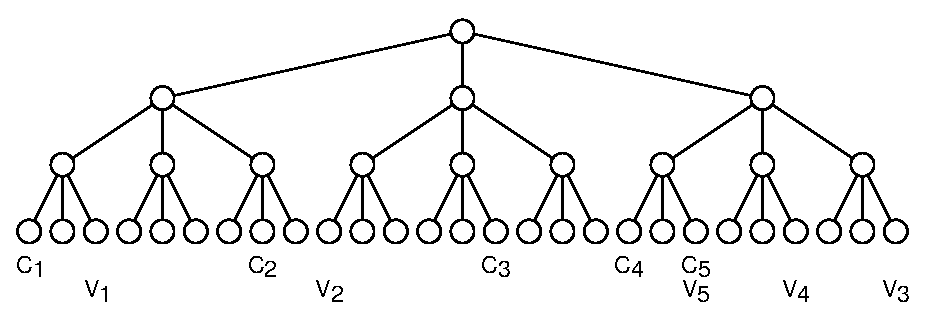
\includegraphics[width = \columnwidth]{figs/basic_scenario_3.eps}
\caption{An example situation with 5 $\Chunk s$ and $\VM s$. Note that $c_5$ and $v_5$ are on the same host.}
\label{fig:model_clean}
\end{figure}



Figure~\ref{fig:model_clean} shows an example situation with $n = 5$. The goal of the $\Problem$  is to find an assignment of the $\VM s$ to the $\Chunk s$, which minimizes the overall bandwidth consumption of the job. 

We will now exemplarically examine an assignment of $\Chunk s$ to $\VM s$. Assume $c_1$ is assigned to $v_1$, $c2$ to $v2$, $c3$ to $v3$, $c4$ to $v4$ and $c5$ to $v5$. Since $v_5$ runs on the same host, which contains $c_5$, transfering $c_5$ to $v_5$ will consume no bandwidth on the physical links. Hence we assume the overall bandwidth costs of the transfer to be $0$. The distrance between $v_1$ and $c_1$ is $2$ hops. Hence the transfer of the $\Chunk$ to the $\VM$ will consume bandwidth on two links. As a result, the overall bandwidth costs is $2 \cdot b_t$, where $b_t$ is the bandwidth neccessary for the transfer of a $\Chunk$. $v_4$ is $4$ hops away from $c_4$, which results in a total cost of $4 \cdot b_t$. Since the hop distance between $v_2$ and $c_2$ is 6, the costs for transferring the $\Chunk$ is $6 \cdot b_t$. The same holds for $v_3$ and $c_3$. The overall bandwidth consumption of the assignment is hence $18 \cdot b_t$. 

This is not an optimal solution for the $\Problem$. To show this, we will inspect a similar mapping. The only difference in the optimal mapping, is that $v_3$ is assigned to $c_2$ and $v_2$ is assigned to $c_3$. The bandwidth costs for transfering $c_2$ to it's assigned $\VM$ do not change, since $v_3$ is still $6$ hops away. $c_3$ however is now only $4$ hops away from its assigned $\VM$, which results in an overall bandwidth consumption of $16 \cdot b_t$.

\subsection{Free $\VM$ Placement - fp}

The Free $\VM$ Placement property describes a variant of our simple model, where the positions of the $\VM s$ are not given in the problem statement but are rather chosen by the described strategy. 

\subsection{Redundant $\Chunk s$ - r}

This property specifies that we have $n$ redundant copies of each $\Chunk$. These copies are entirely equal, and only one instance of a specific chunk type (e.g. $c_1$) has to be read by one $\VM$. Note that we assume $\Chunk s$ to be atomic - they cannot be read from two different locations, requiering only $50\%$ of the bandwidth.

\subsection{Communication Costs - cc}

This model extension accounts for communication costs between the $\VM s$. So far our model accounted bandwidth which is consumed to transfer data from it's location in the physical topology to the $\VM$ which will process it. However, due to the nature of distributed jobs, the $\VM s$ will also comunicate with each other. While we denoted the costs of transfering a chunk over a (1-hop) link with $b_t$, we will refer to the bandwidth costs of transfering data between a pair of $\VM s$ with $b_c$.

\subsection{Bandwidth Constraints - bw}

So far we only focussed on computing minimal bandwidth costs. However, in reality the bandwidth which a single link can offer is limited. This model extension limits the available bandwidth on each physical link $l$ to a value, which is denoted as $TODO FIND SYMBOL$ .
